% Figures for the "Precision first" slide, one page each:
%   1. the default data types: a slider between speed (f32) and precision (f64);
%   2. type promotion: an R value meets an f64 array at f64, at full precision;
%   3. NA handling: R's NA_integer_ is INT_MIN, which {anvl} reports both on the
%      way in and on the way back.
% All three share a 5cm x 3.2cm bounding box. The fourth card, the tail of the
% normal distribution, is plotted in index.qmd.
% Build: pdflatex precision-figures.tex, then
%        pdf2svg precision-figures.pdf precision-<name>.svg <page>
\documentclass[tikz, border=2pt]{standalone}
\usepackage[T1]{fontenc}
\renewcommand{\familydefault}{\sfdefault}
\usetikzlibrary{arrows.meta, shapes.geometric}
\definecolor{accent}{HTML}{107895}
\definecolor{warn}{HTML}{B23B3B}

\tikzset{
  arr/.style={-{Stealth[length=2mm, width=1.6mm]}, thick, draw=black!60},
  lbl/.style={font=\small\itshape, text=black!60},
  cell/.style={draw=black!55, thick, fill=black!5, minimum size=0.42cm, inner sep=0pt,
    font=\ttfamily\small}
}

% A three-cell array whose middle cell is at #1, filled with #2.
\newcommand{\threecells}[2]{
  \node[cell, fill=#2, minimum size=0.4cm] at ($#1 + (-0.4, 0)$) {};
  \node[cell, fill=#2, minimum size=0.4cm] at #1 {};
  \node[cell, fill=#2, minimum size=0.4cm] at ($#1 + (0.4, 0)$) {};
}

\usetikzlibrary{calc}

\begin{document}

% --- 1. speed or precision --------------------------------------------------------
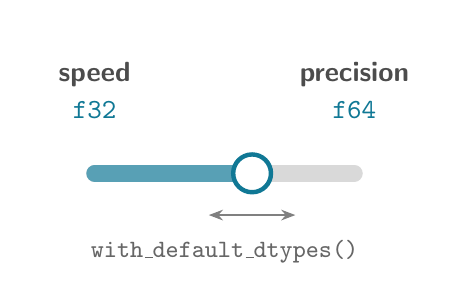
\begin{tikzpicture}
  \path[use as bounding box] (0, 0) rectangle (5.3, 3.2);
  \node[font=\normalsize\bfseries, text=black!70] at (0.85, 2.6) {speed};
  \node[font=\normalsize\bfseries, text=black!70] at (4.15, 2.6) {precision};
  \node[font=\ttfamily\normalsize, text=accent] at (0.85, 2.15) {f32};
  \node[font=\ttfamily\normalsize, text=accent] at (4.15, 2.15) {f64};
  \draw[line width=6pt, black!15, line cap=round] (0.85, 1.35) -- (4.15, 1.35);
  \draw[line width=6pt, accent!70, line cap=round] (0.85, 1.35) -- (2.85, 1.35);
  \fill[white, draw=accent, line width=1.6pt] (2.85, 1.35) circle (0.24);
  \draw[{Stealth[length=1.8mm]}-{Stealth[length=1.8mm]}, thick, black!50] (2.3, 0.82) -- (3.4, 0.82);
  \node[font=\ttfamily\small, text=black!60] at (2.5, 0.35) {with\_default\_dtypes()};
\end{tikzpicture}

% --- 2. type promotion -------------------------------------------------------------
% An R value has no data type of its own: pi meets an f64 array at f64, at full
% precision, instead of being rounded to f32 first.
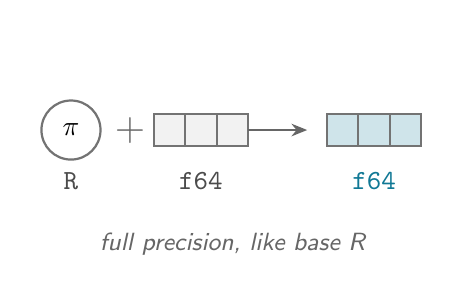
\begin{tikzpicture}
  \path[use as bounding box] (0, 0) rectangle (5.3, 3.2);
  \node[draw=black!55, thick, fill=white, circle, minimum size=0.75cm, font=\normalsize]
    at (0.55, 1.9) {$\pi$};
  \node[font=\Large, text=black!60] at (1.3, 1.9) {+};
  \threecells{(2.2, 1.9)}{black!5}
  \draw[arr] (2.8, 1.9) -- (3.55, 1.9);
  \threecells{(4.4, 1.9)}{accent!20}
  \node[font=\ttfamily\normalsize, text=black!70] at (0.55, 1.25) {R};
  \node[font=\ttfamily\normalsize, text=black!70] at (2.2, 1.25) {f64};
  \node[font=\ttfamily\normalsize\bfseries, text=accent] at (4.4, 1.25) {f64};
  \node[lbl] at (2.6, 0.45) {full precision, like base R};
\end{tikzpicture}

% --- 3. NA handling ------------------------------------------------------------------
% R has no integer NA of its own: NA_integer_ is the bit pattern of INT_MIN.
% {anvl} warns when such a value enters, and when one comes back to R.
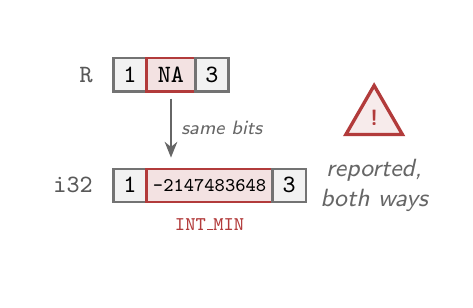
\begin{tikzpicture}
  \path[use as bounding box] (0, 0) rectangle (5.3, 3.2);
  \node[font=\ttfamily\small, text=black!65, anchor=east] at (0.95, 2.6) {R};
  \node[cell] at (1.3, 2.6) {1};
  \node[cell, fill=warn!15, draw=warn, minimum width=0.62cm] at (1.82, 2.6) {NA};
  \node[cell] at (2.34, 2.6) {3};
  \draw[arr] (1.82, 2.3) -- node[right, font=\scriptsize\itshape, text=black!60] {same bits} (1.82, 1.55);
  \node[font=\ttfamily\small, text=black!65, anchor=east] at (0.95, 1.2) {i32};
  \node[cell] at (1.3, 1.2) {1};
  \node[cell, fill=warn!15, draw=warn, minimum width=1.6cm, font=\ttfamily\scriptsize] at (2.31, 1.2) {-2147483648};
  \node[cell] at (3.32, 1.2) {3};
  \node[font=\ttfamily\scriptsize, text=warn] at (2.31, 0.7) {INT\_MIN};
  \node[draw=warn, fill=warn!10, regular polygon, regular polygon sides=3, inner sep=1.4pt,
    line width=1.2pt, font=\bfseries\footnotesize, text=warn] at (4.4, 2.05) {!};
  \node[lbl, align=center] at (4.4, 1.2) {reported,\\both ways};
\end{tikzpicture}

\end{document}
